\documentclass[10pt,a4paper]{article}
\usepackage[spanish,english]{babel}
\usepackage{indentfirst}
\usepackage{anysize} % Soporte para el comando \marginsize
%\marginsize{1.5cm}{1.5cm}{0.5cm}{1cm}
\marginsize{2,5cm}{1,8cm}{1.5cm}{1,7cm}
\usepackage[psamsfonts]{amssymb}

\usepackage{amssymb}
\usepackage{amsfonts}
\usepackage{amsmath}
\usepackage{amsthm}
\usepackage{multicol}
\usepackage{multirow} 
\usepackage{graphicx}
\usepackage{hyperref}
\usepackage{caption}
\usepackage{float}
\usepackage{subcaption}
\usepackage{tocloft}
\usepackage{listings}
\renewcommand{\cftsecleader}{\cftdotfill{\cftdotsep}}
\renewcommand*\contentsname{Summary}
\renewcommand{\thepage}{}
\theoremstyle{definition}
\renewcommand{\thefootnote}{\fnsymbol{footnote}}

\begin{document}
	
\title{Multithreaded Battle City Console Game}
\date{5/07/2020}
\maketitle

\begin{center}
	Students:\\
	\vspace{5pt}
	{\large ALEGRE IB\'A\~NEZ, V\'ictor Augusto 20130504C

ZAVALETA BUENO, Romel Rolando 20120236F

ZEVALLOS LABARTHE, Enrique Mart\'in 20130384H}\\
	Universidad Nacional de Ingenier\'ia, Facultad de Ciencias,\\
	e-mail: victoralegre@uni.pe, romelzavaleta@uni.pe, enrique.zevallos.l@uni.pe
	
\end{center}
\vspace{5pt}
\begin{center}
	Subject:\\
	\vspace{5pt}
	{\large CC462 - Concurrent \& Distributed Systems
}\\
	{\large Lab 2}\\
	

	
\end{center}
\vspace{20pt}
\begin{abstract}
{\small
\hspace*{0.5cm}
	In this laboratory, we will develop the well-known game \textit{Battle City} implementing a client-server model. We opted for a distributed and concurrent approach where both server and client implement threads to optimize performance. The server will continuously listen for new connections and will be in charge of most of the processing needed. Clients will only have to worry about the GUI and after establishing the connection with the server, send keystrokes and receive the data needed to re-draw the map and the tanks (other clients and themselves) within.\\\\
\textbf{Keywords:} Threads, Concurrency, Distributed, Console, Game, Battle, City.
}
\end{abstract}



\pagenumbering{arabic}

\tableofcontents

\vspace{20pt}
\hrule
\vspace{10pt}

\section{Introduction}
The notion of client-server models has been used extensively throughout the gaming industry. 
This allows distributed processing of the payload, such that the client will only have to execute a lightweight version of the program. 
The vast majority of the processing is done by the server. 
Clients are only in charge of sending orders for the server to execute, and creating and updating the GUI. 
In this particular instance, we have developed the logic of the game within a server, to which several clients will connect to play. 
The server is in charge of updating the map with the information it receives from the clients. 
Clients will conect to the server and send keystrokes in order to shoot and move within the map. 
The server will then return the updated map for the client to draw.
This way, the client can run in a wider variety of hardware choices with similar performance.


\section{Theoretical Framework}
For the implementation of the game, we are using a multithreaded approach in both the client and the server. 
The server will use a thread for each new player that asks to connect. 
Its implementation consists of two infinite loops. 
One of them waits for new connections, and the other sends updates (in 100 millisecond intervals) of the players' positions, shots and collisions. 
Players are objects stored in a list and instantiated using a network socket. 
This socket will provide both input and output streams for the client keystrokes and map characters, respectively. 
Additionally, players will have a list of \textit{bullet} objects. 
Both players and bullets will have attributes of position in a 2D "battle ground". 
The instantiated server will iterate over all player objects to determine their direction and movements. 
If the coordinates of a bullet are the same as those of a player, then this player will be eliminated. 
For the client, only two threads are implemented. 
The main thread is in charge of the GUI and event handling from keystrokes. 
The other thread will read the output from the server, either map updates or an "eliminated" notification.

\section{Methodolody}
\subsection{The Server}
The server implementation is made in our main class, which instantiates the \textit{ServerThread} class in a \textit{server} object, and calls its methods \textit{start} and \textit{enviarUpdates}. 
This class inherits from the \textit{Thread} class and so it implements a runnable method when \textit{start} is called. 
In this case, we overrode the \textit{run} method to run an infinite loop and wait for new connections. 
After establishing a new connection, a player object named \textit{jugador} is instantiated using the class \textit{ServerJugador} which also inherits from the \textit{Thread} class. \\
The spawning position of the new object is generated randomly. 
This new object is added to the list \textit{jugadores} and then \textit{jugador.start()} will call its runnable method. 
The \textit{run} method is overridden to establish two data streams, input and output. 
We use a \textit{while} loop that checks if the \textit{running} attribute is still \textit{true}. 
This value is modified to be set as \textit{false} when the \textit{notificaPerdido} method is called, after the player object (\textit{jugador}) is added to the \textit{gamer\_eliminado} list, when its position is the same as that of a bullet. \\
This loop keeps on reading the input stream if \textit{running} is set to \textit{true}, as well as establishing the object's movement and determining if shots were fired. 
If the \textit{key} it receives from the input stream is \textit{'x'}, then it will instantiate a bullet (\textit{bala}) object. 
This bullet will receive its initial coordinates from the player that instantiated it, its state is set to true and it is added to the \textit{balas} list of objects. \\
Another method of the \textit{ServerJugador} class is \textit{enviar}, which sends a message in UTF-8 encoding through the output stream. 
This method will be called from the \textit{server} object to send the updated map to the client. 
After the player is instantiated and initialized in the server's runnable method, the method \textit{enviarUpdates} is called. 
This method creates a thread and calls its runnable method where an infinite loop updates the total amount of players and creates a list of eliminated players. 
It sleeps for 100 milliseconds, then prints the number of players and coordinates of a collision. 
If there were no collisions, the coordinates will be (0,0). \\
Then a \textit{for} loop iterates over the list of players and for each one of them, it will call the \textit{CoreJuego} method which modifies the orientation and position based on the \textit{direccion} attribute of the player. 
It will also check for bullets, determining its movements and collisions. 
If the object it collides with is a 'tank', the collision coordinates are modified and thus the condition in the next line of code will verify.
After the player is passed to the method \textit{CoreJuego}, and the physics of the game is implemented, we use an \textit{if} statement to determine if a bullet collided with a 'tank', and proceed to add said player to the \textit{gamer\_eliminado} list of objects. 
The collision coordinates are then set back to (0,0). 
Then, after exiting the if condition the method \textit{enviar} is called for each player, and the \textit{for} loop finishes. \\
Finally, we iterate over the \textit{gamer\_eliminado} list and call the method \textit{notificaPerdio} to send the notification \textit{"pierdes"} through the output stream, and set the \textit{running} attribute of the player to \textit{false}. 
All disqualified players are remove and the thread sleeps for an additional 100 milliseconds.
The last class we ought to mention is \textit{CargarMapa}. 
This class will create a 16x32 matrix reading each string of the \textit{mapa.txt} file. 
If any exception should be thrown, the appropriate \textit{try} and \textit{catch} statements are in place. 
A \textit{while} and a \textit{for} loop are implemented to iterate over the whole text file and populate the map matrix.
\subsection{The Client}
As mentioned, the client will run two threads. 
One of them will be in charge of the GUI and event handling from keystrokes. 
The GUI is implemented using the Swing library from Java. 
An object called \textit{Marco} which inherits from JFrame is instantiated where the width, height and title are already specified. 
Then several methods are called to set the default close operation to exit on close, set the frame to visible and non-resizable.
Another object called \textit{inicio} is instantiated from the class \textit{InicioPanel} which inherits from JPanel. 
This class has the attributes of host and port as JTextFields and implements an ActionListener for the \textit{Jugar!!} button. 
When this button is pressed the client will connect to the specified host, at the specified port, calling the \textit{jugar} method. 
This method creates the object \textit{juego} using the class \textit{JuegoPanel} which also inherits from the class JPanel. \\
Then the \textit{startGame} method from the \textit{juego} object is called, and within this piece of code an object called \textit{socketThread} is instantiated using the \textit{SocketThread} class. 
This class inherits from the Thread class, and uses network sockets to connect to the server. 
It will also have input and output datastreams, and a \textit{running} attribute set to true initially. 
The thread will implement a runnable method with a \textit{while} loop that verifies if the message sent from the server is \textit{pierdes}. 
This message is read using the \textit{leer} method where a conditional statement waits for the specific message telling the client it lost, in order to activate the listener's \textit{notificaPerdio} method. 
If so, the listener will set the value of \textit{running} to false, and the loop will stop running.
After this \textit{if} statement, the \textit{repintar} method is called which essentially is a \textit{setText} command to re-draw the playing field. 
If we were to exit the \textit{while} loop, the runnable implements \textit{try}, \textit{catch} and \textit{finally} clauses to print out error messages in case the connection is lost and the socket ought to be closed. 
The output stream will have a method called \textit{enviarOrden} that will be called from the JuegoPanel class.\\
After the game is started, a Key Listener will listen to keystrokes from the client and send them through the output stream. It uses the method named \textit{mandarOrden} to perform a \textit{switch-case} specifying the possible commands that the client can use. 
This piece of code is the reason why in the client you use the space-bar to shoot, but the server interprets this as an 'x' character, since it is easier than implementing the use of the empty character ' '. 
Other methods in JuegoPanel will be in charge of notifying the player of possible errors or losing the game.

\section{Results and Discussion}
After testing the game with several clients connecting simultaneously to the deployed server code in a cloud based service (AWS), 12 players were able to play within the same field with very little lag time. 
Some issues we encountered had to do with the bullets killing the tanks that fired them, and stopping if the tank moved in the same direction. 
The latter is due to the fact that when created, the map has to be redrawn with the tank inside or otherwise the tank will disappear due to the bullet it just shot.

\begin{figure}[H]
	\centering
	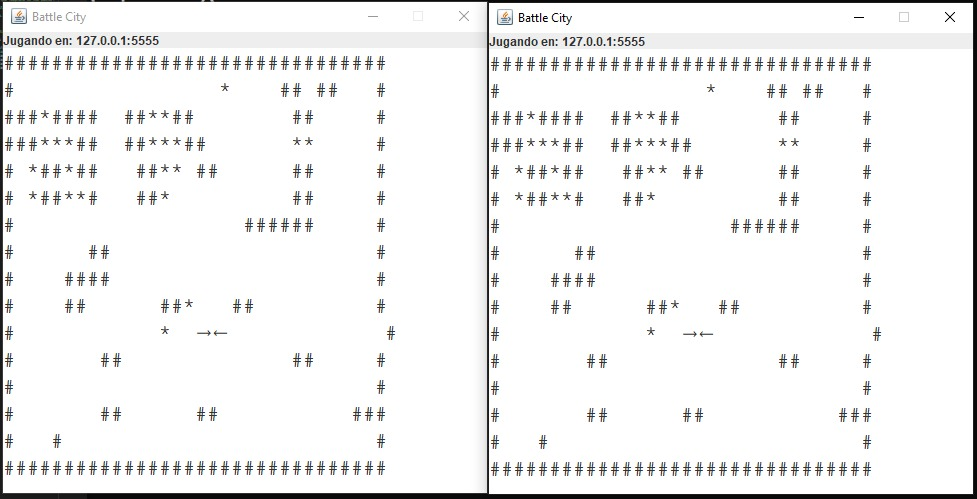
\includegraphics[width=0.75\textwidth]{battle.jpg}
	\caption{BattleCity with two players}
	\label{fig:battlecity}
\end{figure}

In the example we implemented (found in our GitHub \href{https://github.com/ezevallos/CC462_Battle-City}{Repository}), we include both source code for the classes implemented, as well as the executable jars for the user to run.

\section{Conclusions}
The implementation of multithreading will allow us to improve the performance of the BattleCity game. 
The use of a distributed client-server setup allows lightweight client-side applications. 
This makes the solution scalable, if more computational power is needed, the resources within the web service are scaled up to meet the requirements. 

\section{Code}
The code is in the following link \url{https://github.com/ezevallos/CC462_Battle-City}
%\section{Anexo Documentación}


%\begin{center}
%{\large \bf Agradecimientos}
%\end{center}
%Los autores agradecen a las autoridades de la Facultad de Ciencias de la Universidad Nacional de 
%Ingenier\'{\i}a por su apoyo.
%%\begin{center}
%%{\large \bf Apendice: }
%%\end{center}

\vspace{20pt}
\hrule
\vspace{10pt}

\nocite{*}
%\bibliographystyle{apacite}
\bibliographystyle{plain}
\bibliography{Bibliog}
\addcontentsline{toc}{chapter}{Bibliografía}

%------------------------------------- References --------------------
\end{document}
